\documentclass[10pt, legalpaper, twoside]{article}\usepackage[]{graphicx}\usepackage[]{color}
% maxwidth is the original width if it is less than linewidth
% otherwise use linewidth (to make sure the graphics do not exceed the margin)
\makeatletter
\def\maxwidth{ %
  \ifdim\Gin@nat@width>\linewidth
    \linewidth
  \else
    \Gin@nat@width
  \fi
}
\makeatother

\definecolor{fgcolor}{rgb}{0.345, 0.345, 0.345}
\newcommand{\hlnum}[1]{\textcolor[rgb]{0.686,0.059,0.569}{#1}}%
\newcommand{\hlstr}[1]{\textcolor[rgb]{0.192,0.494,0.8}{#1}}%
\newcommand{\hlcom}[1]{\textcolor[rgb]{0.678,0.584,0.686}{\textit{#1}}}%
\newcommand{\hlopt}[1]{\textcolor[rgb]{0,0,0}{#1}}%
\newcommand{\hlstd}[1]{\textcolor[rgb]{0.345,0.345,0.345}{#1}}%
\newcommand{\hlkwa}[1]{\textcolor[rgb]{0.161,0.373,0.58}{\textbf{#1}}}%
\newcommand{\hlkwb}[1]{\textcolor[rgb]{0.69,0.353,0.396}{#1}}%
\newcommand{\hlkwc}[1]{\textcolor[rgb]{0.333,0.667,0.333}{#1}}%
\newcommand{\hlkwd}[1]{\textcolor[rgb]{0.737,0.353,0.396}{\textbf{#1}}}%
\let\hlipl\hlkwb

\usepackage{framed}
\makeatletter
\newenvironment{kframe}{%
 \def\at@end@of@kframe{}%
 \ifinner\ifhmode%
  \def\at@end@of@kframe{\end{minipage}}%
  \begin{minipage}{\columnwidth}%
 \fi\fi%
 \def\FrameCommand##1{\hskip\@totalleftmargin \hskip-\fboxsep
 \colorbox{shadecolor}{##1}\hskip-\fboxsep
     % There is no \\@totalrightmargin, so:
     \hskip-\linewidth \hskip-\@totalleftmargin \hskip\columnwidth}%
 \MakeFramed {\advance\hsize-\width
   \@totalleftmargin\z@ \linewidth\hsize
   \@setminipage}}%
 {\par\unskip\endMakeFramed%
 \at@end@of@kframe}
\makeatother

\definecolor{shadecolor}{rgb}{.97, .97, .97}
\definecolor{messagecolor}{rgb}{0, 0, 0}
\definecolor{warningcolor}{rgb}{1, 0, 1}
\definecolor{errorcolor}{rgb}{1, 0, 0}
\newenvironment{knitrout}{}{} % an empty environment to be redefined in TeX

\usepackage{alltt}
% font size could be 10pt (default), 11pt or 12 pt
% paper size coulde be letterpaper (default), legalpaper, executivepaper,
% a4paper, a5paper or b5paper
% side coulde be oneside (default) or twoside 
% columns coulde be onecolumn (default) or twocolumn
% graphics coulde be final (default) or draft 
%
% titlepage coulde be notitlepage (default) or titlepage which 
% makes an extra page for title 
% 
% paper alignment coulde be portrait (default) or landscape 
%
% equations coulde be 
%   default number of the equation on the rigth and equation centered 
%   leqno number on the left and equation centered 
%   fleqn number on the rigth and  equation on the left side
%	

\usepackage{graphicx}
\usepackage{url}
\usepackage{hyperref}

\title{Interactive Graphics for Visually Diagnosing Forest Classifiers in R}
\author{Natalia da Silva\thanks{Corresponding Author}  \\
	    Instituto de Estad\'istica (IESTA), Universidad de la Rep\'ublica\\ Email:  natalia@iesta.edu.uy\\
	\and 
	Dianne Cook \\
	Department of Econometrics and Business Statistics, Monash University\\ Email:dicook@monash.edu \\
		\and 
		Eun-Kyung Lee\\
		Department of Statistics,  Ewha Womans University \\
		Email:lee.eunk@gmail.com
	}

\date{} 
% \date{\today} date coulde be today 
% \date{25.12.00} or be a certain date
% \date{ } or there is no date
\IfFileExists{upquote.sty}{\usepackage{upquote}}{}
\begin{document}
% Hint: \title{what ever}, \author{who care} and \date{when ever} could stand 
% before or after the \begin{document} command 
% BUT the \maketitle command MUST come AFTER the \begin{document} command! 
\maketitle

\begin{abstract}
This article describes structuring data and constructing plots to explore forest classification models interactively. A forest classifier is an example of an ensemble since it is produced by bagging multiple trees. The process of bagging and combining results from multiple trees produces numerous diagnostics which, with interactive graphics, can provide a lot of insight into class structure in high dimensions. Various aspects are explored in this article, to assess model complexity, individual model contributions, variable importance and dimension reduction, and uncertainty in prediction associated with individual observations. The ideas are applied to the random forest algorithm and projection pursuit forest, but could be more broadly applied to other bagged ensembles. Interactive graphics are built in R using the \texttt{ggplot2}, \texttt{plotly}, and \texttt{shiny} packages.
\end{abstract}

%\tableofcontents % create a table of contens 


\section{Introduction}
The random forest (RF) algorithm \cite{breiman1996bagging} was one of the first ensemble classifiers developed.  It combines the predictions from individual classification and regression trees (CART) \cite{breiman1984cl} built by bagging observations \cite{breiman1996bagging}. It also samples variables at each tree node. These produce diagnostics in the form of uncertainty in predictions for each observation, importance of variables for the prediction, predictive error for future samples based on out-of-bag (oob) case predictions, and similarity of observations based on how often they group together in the trees.

Ensemble classifiers have grown in popularity \cite{dietterish00} \cite{talbot09}, and the basic ideas behind the random forest can be applied to virtually any type of model. The benefits for classification are reduced variability in predictive error, and the suite of diagnostics provides the potential for better understanding the class structure in the high-dimensional data space. The use of visualization on these diagnostics, in association with multivariate data plots, completes the process to support a better understanding of the underlying problem.

A conceptual framework for model visualization can be summarized in three strategies: (1) visualize the model in the data space, (2) look all members of a collection of a model and (3) explore the complete process of model fitting \cite{wickham2015visualizing}. The first strategy is to explore how well the model captures the data characteristics (model in the data space), which contrasts with determining if the model assumptions hold (data in the model space). The second strategy is to look at a group of models instead of only the best model. This strategy can offer a broad understanding of the problem by comparing and contrasting possible models. The last strategy focuses on exploring the process of the model fitting in addition to the end result.

There has been some, but not a lot of, research on visualizing classification models.
\cite{urbanek2002exploring} presents interactive tree visualization implemented in the java software called  \texttt{KLIMT} that include zooming, selection, multiple views, interactive pruning, and tree construction as well as the interactive analysis of forests of trees using treemaps. \cite{cutler15raft} developed a java package called \texttt{RAFT} to visualize a forest classifier, that included variable selection, parallel coordinate plots, heat maps, and scatter plots of some diagnostics. Linking between plots is limited. \cite{quach2012interactive} presents interactive forest visualization using the R package \texttt{ iPlots eXtreme}  \cite{urbanek2011iplots} where several displays are shown in one window with some linking between them available. \cite{Silva2016} describes visualizing components of an ensemble classifier.

This article describes structuring interactive graphics to facilitate visual exploration of ensemble classifiers using RFs and projection pursuit random forests (PPF) \cite{da2021projection} as examples. The PPF algorithm builds on the projection pursuit tree (PPtree) \cite{lee2013pptree} algorithm which uses projection pursuit at each tree node to find the best linear combination of variables to separate the classes. The visualization approach is consistent with the framework in \cite{wickham2015visualizing}, and the implementation is built on the newest interactive graphics available in R \cite{RCore}. The purpose is to provide readily available tools for users to explore and improve ensemble fits and obtain an intuition for the underlying class structure in data. Interactive plots are a key component for model visualization that help the user see multivariate relationships and be more efficient in the model diagnosis. Multiple levels of data are constructed for exploration: observation, model and ensemble summaries.

The article is structured as follows.  Section \ref{visen} describes the ensemble components to be accessed and how to map components to visual elements. The web app is described in \ref{app} and further work is discussed in section \ref{fur}.

\section{Mapping Ensemble Diagnostics to Visual Components}~\label{visen}
This section describes the ensemble components and the mapping of diagnostics to visualizations. These are illustrated using the Australian crabs data \cite{CM74}. 

In forest classifiers some diagnostics typically available are:

\begin{itemize} \itemsep 0in
\item {\em Out-of-bag error:}  is a measure for each model that is combined in the ensemble and is used to provide the overall error of the ensemble.
  
\item {\em Uncertainty measure for each observation:} Across individual (classification) models  the proportion of times that a case is predicted to be in each class can be computed. 

\item {\em Variable importance:} Each model uses samples of variables. So that, the accuracy of the models can be compared when the variable is included or omitted. There are several versions of statistics that use this to provide a measure of the variable importance for prediction.

\item {\em Similarity measure for pairs of observations:} In each model, each pair of observations will be either in the same terminal node or not. This is used to compute a proximity matrix. 
\end{itemize}

In addition to these overall ensemble statistics, each individual model has its own diagnostics, measuring error, variables utilized, and class predictions. Visualization will enable the individual models to be examined, relate these to the data and their contribution to the ensemble.

Australian crabs data are used to describe the diagnostics. The data has 200 cases, 5 predictors and 4 classes (combinations of species and sex, blue male, blue female, orange male and orange female). The predictors are: FL (the size of the frontal lobe length, in mm), RW (rear width, in mm), CL (length of mid-line of the carapace, in mm), CW (maximum width of carapace, in mm), BD (depth of the body; for females, measured after displacement of the abdomen, in mm). This is old data, but it provides a good illustration of the visual methods.


\subsection{Individual Models: PPtree}

The PPF is composed of individual projection pursuit trees. Figure \ref{pptreeviz1} shows a visual ensemble of plots of a tree model on the crab data. There are three nodes for the four class problem. The nodes of this tree are based on projections of the data; the coefficients of which form the building block to calculate the variable importance. The density plot displays the data projection at each node, and the mosaic plot shows the confusion matrix for the nodes.
The package \texttt{PPtreeViz} provides visual tools to diagnose a PPtree model. The PPF builds on these and modifies a little. The PPtree model is simpler than a regular classification tree because the classes are mostly separated by combinations of variables -- just three projections are needed to see the differences between the four classes.





\begin{figure}[hbpt]
\centering
\begin{knitrout}
\definecolor{shadecolor}{rgb}{0.969, 0.969, 0.969}\color{fgcolor}

\includegraphics[width=\maxwidth]{figure/trcomb-1} 


\includegraphics[width=\maxwidth]{figure/trcomb-2} 
\end{knitrout}
\caption{Visualizing the PPtree model of the crab data. The tree has three nodes (top). The density plots show the data projections at each node, colored by group (middle). The dashed vertical red line indicates the split value of each node. At node 1 the blue species is separated from orange species. Nodes 2 and 3 separate the sexes, which are more confused for the blue species. Mosaic plots of the confusion table for each split (bottom). Node 1 shows the clear split of the species, with a small number of misclassifications. Node 2 where orange females are separated from orange males indicates small number of misclassifications. Node 3 where blue females are separated from blue males, shows a larger misclassification than for orange specie.\label{pptreeviz1}}
\end{figure}




\subsection{Variable Importance}

The PPF algorithm calculates variable importance in three ways: permuted importance using accuracy,  and two importance measures based on projection coefficients on standardized variables.

The first importance measure is comparable with the measure defined in the classical random forest algorithm. Importance variable is computed based on the oob cases for the tree $k\;\;(O_k)$ for each $j$ predictor variable.
Permuted importance of the variable $j$ in the tree $k$ is defined as:

\[
VI^{(1)} _{jk} = \frac{\sum_{i \in O_k } I(y_i=\hat y_{ik})-I(y_i=\tilde y_{ik})}{\# O_k}
\]

\noindent where $\hat y_{ik}$ is the predicted class for the observation $i$ in the tree $k$, and $\tilde y_{ik}$ is the predicted class for the observation $i$ in the tree $k$ after permuting the values for variable $j$. The global permuted importance measure is the average importance over all the trees in the forest. This measure is based on comparing the accuracy of classifying oob observations using the true class with permuted (nonsense) class.

The coefficients of each projection are examined to define the other two importance measures. If the variables have been standardized, the magnitude of these values indicates importance. For a single PPtree the variable importance is computed by a weighted sum of the absolute values of the coefficients across node, then the weights take the number of classes in each node into account($G_s$) \cite{lee2013pptree}.

The global variable importance in a PPforest then can be defined in different ways. One way is to average the variable importance from each PPtree across all the trees in the forest. Alternatively, can be computed as a weighted mean of the absolute value of the projection coefficients across all nodes in every tree, for more details \cite{da2021projection}.

Figure \ref{impotree} shows the absolute projection coefficient of the top three nodes for all the trees in a forest model. This information is displayed by a side-by-side jittered dot plot. The red dots correspond to the absolute coefficient values for the tree model of Figure \ref{pptreeviz1}. The forest was built using random samples of two variables for each node, hence there are two coefficients for each node. At node 1, BD has a high value and CW contributes much less. The scatterplot at right shows these two variables and the resulting boundary between groups that this would produce. Node 2 uses CL and RW, and RW contributes the most to the separation. The plot at right shows the boundary that is induced. Node 3 uses FL and RW, and this is a much more even contribution by the two variables.
For each tree in the forest, different decision rules are defined; the resulting boundaries on the previous plots are based on Rule 1 $= \frac{m_1}{2} + \frac{m_2}{2} $, where $m_1$ and $m_2$ are the mean of the left and right groups at each node.

\begin{figure}[hbpt]
\centering
\begin{knitrout}
\definecolor{shadecolor}{rgb}{0.969, 0.969, 0.969}\color{fgcolor}

\includegraphics[width=\maxwidth]{figure/treenode-1} 
\end{knitrout}
\caption{Visualizing the variable importance of all the trees in the forest, for three nodes. Each node of each tree has an importance value for each variable. The values for the whole forest are displayed using a side-by-side jittered dot plot. The importance values are the absolute values of the projection coefficients. The red points correspond to these values for the tree shown in Figure \ref{pptreeviz1}. Two variables are randomly selected at each node for creating the best projection, and split. The plots are right show the variables used and the split made at each of the nodes of this tree.  \label{impotree}}
\end{figure}

\subsection{Similarity of Cases}

For each tree, every pair of observations can be in the same terminal node or not. Tallying this up across all trees in a forest gives the proximity matrix, an $n\times n$ matrix of the proportion of trees that the pair share a terminal node. It can be considered a similarity matrix.

Multidimensional scaling (MDS) is used to reduce the dimension of this matrix, to view the similarity between observations. MDS transforms the dataset into a low-dimensional space where the distances are approximately the same as in the full $n$ dimensions. With $G$ groups, the low-dimensional space should be no more than $G-1$ dimensions. Figure \ref{prox1} shows the MDS plots for the three dimensional space induced by the four groups of the crab data. Color indicates the true species and sex. For this data two dimensions are enough to see the four groups separated quite well. Some crabs are clearly more similar to a different group, especially in examining the sex differences.
\begin{figure}[hbpt]
\centering
\begin{knitrout}
\definecolor{shadecolor}{rgb}{0.969, 0.969, 0.969}\color{fgcolor}

\includegraphics[width=\maxwidth]{figure/mds-1} 
\end{knitrout}
\caption{Examining similarity between cases, using pairwise plots of multidimensional scaling into three dimensional. It can be seen that most cases are grouped closely with their class, and particularly that the two species are distinct. There is more confusion of cases between the sexes. \label{prox1}}
\end{figure}


\subsection{Uncertainty of Cases}

The vote matrix ($n \times G$) contains the proportion of times each observation was classified to each class while oob. Two approaches to visualize the vote matrix information are used.

A ternary plot is a triangular diagram used to display compositional data with three components. More generally, compositional data can have any number of components, say $p$, and hence is constrained to a $(p-1)$ dimensional simplex in $p$-space. The vote matrix is an example of compositional data with $G$ components.

With G classes, the ternary plot idea is generalized to a $(G-1)- dimensional$ simplex \cite{sutherland2000orca, schloerke}. This is one of the approaches used to visualize the vote matrix.

For the crab data, $G=4$ and the generalized ternary plot will be a tetrahedron. The  \texttt{tourr} package \cite{wickham2011tourr} can be used to view it (e.g. \url{https://vimeo.com/170522736}).

Figure \ref{tetra} shows the tetrahedron structure for the crab vote matrix shown in three pairwise views. With well-separated classes, the colored points will each concentrate into one of the vertices. This is close but not perfect, indicating some crabs are commonly incorrectly predicted.
\begin{figure}[hbpt]
\centering
\begin{knitrout}
\definecolor{shadecolor}{rgb}{0.969, 0.969, 0.969}\color{fgcolor}

\includegraphics[width=\maxwidth,trim=0cm 2cm 0cm 2cm, clip]{figure/ternary-1} 
\end{knitrout}
\caption{Generalized ternary plot ((G-1) dimensional simplex, here it is a tetrahedron) representation of the vote matrix for four classes. The tetrahedron is shown pairwise. Each point corresponds to one observation and color is the true class. This is close but not a perfect classification, since the colors are concentrated in the corners and there are some mixed colors in each corner.}
\label{tetra}
\end{figure}

Because visualizing the vote matrix with a $(G-1)$ dimensional tetrahedron requires dynamic graphics, a low-dimensional option is also provided. For each class, each case has a value between 0-1. A side-by-side jittered dotplot is used for the display, where class is displayed on one axis and proportion is displayed on the other. It is not as elegant as the ternary plot, but it is useful because it places focus on each group. Each dotplot shows the proportion of times the case was predicted into the group, with 1 indicating that the case was always predicted to the group and 0 being never. For each dotplot, the ideal arrangement is that points are concentrated at 0 or 1 and only at 1 for their true class. This data is close to the ideal but not perfect, e.g. there are a few blue male crabs (orange) that are frequently predicted to be blue females (green), and a few blue female crabs predicted to be another class(See Figure in the first \verb tabPanel  at \href{https://natydasilva.shinyapps.io/shinyppforest}{PPforestApp}). 

% \begin{figure}[hbpt]
% \centering
% <<side, echo=FALSE, warning=FALSE, message=FALSE, fig.height=3.5,fig.width=3.5>>=
% 
% #side-by siede boxplot
% side <-  function(ppf, ang = 0, lege = "bottom", size = 3,
%                   ttl = "Side by side dotplot") {
%   voteinf <- data.frame(ids = 1:length(ppf$train[, 1]), Type = ppf$train[, 1],
%                       ppf$votes, pred = ppf$prediction.oob ) %>%
%   gather(Class, Probability, -pred, -ids, -Type)
% 
%   ggplot(data = voteinf, aes(Class, Probability, color = Type)) +
%     geom_jitter(height = 0, size = I(siz), alpha = .5) +
%     ggtitle(ttl) +
%     scale_colour_brewer(type = "qual", palette = "Dark2") +
%     theme(legend.position = lege, legend.text=element_text(angle = ang)) +
%     labs(colour = "Class", y = "Proportion")
% }
% 
% 
% side(ppf, ttl="")
% 
% @
% \caption{Another representation of the vote matrix, as a jittered side-by-side dotplot. It is not as elegant as the ternary plot, but it is useful because it places focus on each group. Each dotplot shows the proportion of times the case was predicted into the group, with 1 indicating that the case was always predicted to the group and 0 being never. On each dotplot, a single color dominates the top, indicating fairly clear distinctions between classes. Crabs from the blue species, both male and female, have more uncertainty in predictions, as seen by more crabs from other classes having higher vote proportions, than is seen in the orange species.}
% \label{sideby}
% \end{figure}

\section{Interactive Web App }\label{app}
%Todo the PPforestViz pakage

 Interaction is added to the plots described in Section \ref{visen} and other plots, and they are organized into an interactive web app using \texttt{shiny} \cite{chang11shiny} for exploring the ensemble model. The app is organized into three tabs: individual cases; models; and performance comparison, to provide a model diagnostic tool. Interaction is provided as mouse-over labeling, mouse-click selection, and brushing, with results linked across multiple plots. The app takes advantage of new tools provided in the \texttt{plotly} \cite{plotly} package, developed as a part of Sievert's PhD thesis research \cite{sievertthesis}.

The \texttt{plotly} functions directly translate a static \texttt{ggplot2} object by  extracting  information  and  storing it in JavaScript Object Notation (JSON). This information is passed as input to a javascript function to produce a web graphic.  Interactions in a single display, and links between different graphics are two key tasks an interactive visualization should accomplish \cite{xie2014reactive}.

As \cite{sievert2020interactive} describes, one of the biggest difficulties for the app in order manage linking between plots is the data structure management for each widget. Each widget has it own data structure and interaction. Putting them into the structure of a shiny app facilitates access to the widget data and coordinates selections across multiple plots.

The fishcatch data \cite{fishcatch} is used to illustrate the shiny app characteristics. It contains 159 observations, with 6 physical measurement variables, and  7 types of fish, all caught from the same lake (Laengelmavesi) near Tampere in Finland. There are 35 bream, 11 parkki, 56 perch, 17 pike, 20 roach, 14 smelt and 6 whitewish. The shiny app showing fishcatch data can be accessed at \href{https://natydasilva.shinyapps.io/shinyppforest}{PPforestApp}.

\subsection{Individual Cases}

This tab is designed to examine uncertainty in the classification of observations and to explore the similarity between pairs of observations. The data feeding the display is an $n\times p$ data frame, containing the original data, the model statistics generated from the full $n\times G$ vote matrix along with its generalized ternary coordinates, and the first two MDS projections of the proximity matrix.
The first \verb tabPanel  in the \href{https://natydasilva.shinyapps.io/shinyppforest}{PPforestApp} shows the arrangement of plots.
The plots in the tab are (1) a parallel coordinate plot (PCP) of the data, (2) the MDS display of the proximity matrix, (3) side-by-side jittered dotplot, and (4) generalized ternary plot of the vote matrix. Each of these plots are interactive in the sense that each one presents individual interactions (mouse-over) and they are linked so that selections in one display are propagated to other plots (clicking and selecting).

This selection of plots enables aspects of the model, relating to performance for individual cases, to be examined in the data space. The data plot is an essential element following the {\em model-in-the-data-space} philosophy of \cite{wickham2015visualizing}. The choice was made to use a parallel coordinate plot because it provides a space-efficient display of the data. Alternatives include the tour, a dynamic plot, or a scatterplot matrix. Theoretically, either of these could be substituted or added.

% \begin{figure}[hbpt]
% \centering
% \includegraphics[width=1\linewidth]{figure/fish11.png}
% \caption{Entry page for the web app, focusing on examining cases, in terms of similarity and uncertainty. The top plot shows the data, the remaining plots show similarity of cases and uncertainty in predictions. All of the plots are linked, so that selecting elements of one will generate changes in the others. \label{tab1}}
% \end{figure}

The diagram in Figure \ref{tab1diag} illustrates the data pipeline \cite{BAHM88,wickham2009plumbing} for the interactive graphics in the case level tab. Solid lines indicate notifications from the source data to the plots, and dashed lines indicate notification of user action on the plot, that notifies the data source of actions to take. The data table is a reactive object that has a listener associated with it. Each of the plots is reactive and has numerous listeners. When users make selections on a plot, either by clicking or group selection, a change to the data is made in terms of an update on the selected cases. This invokes a note to other plots to re-draw themselves. The linking between plots is effectively one-to-one, based on the row id of the data. The side-by-side jittered dotplot has $n\times G$ points, but selection can only be done within a dotplot. Selecting in one of the dotplots notifies the data table of the selection which triggers a re-draw of the other dotplots. Mouseovers on the plot pull additional information about the point or line under the cursor but doesn't link between plots.

Two alternatives can be selected in shiny to draw the parallel coordinate plot: parallel or enhanced. Parallel draws the classic PCP and enhanced draws a modified version where variables are repeated \cite{hurley2011eulerian}.  Because reading a PCP is really only possible for neighboring variables, the variables are repeated so that all variables are neighboring.

\begin{figure}[hbpt]
\centering
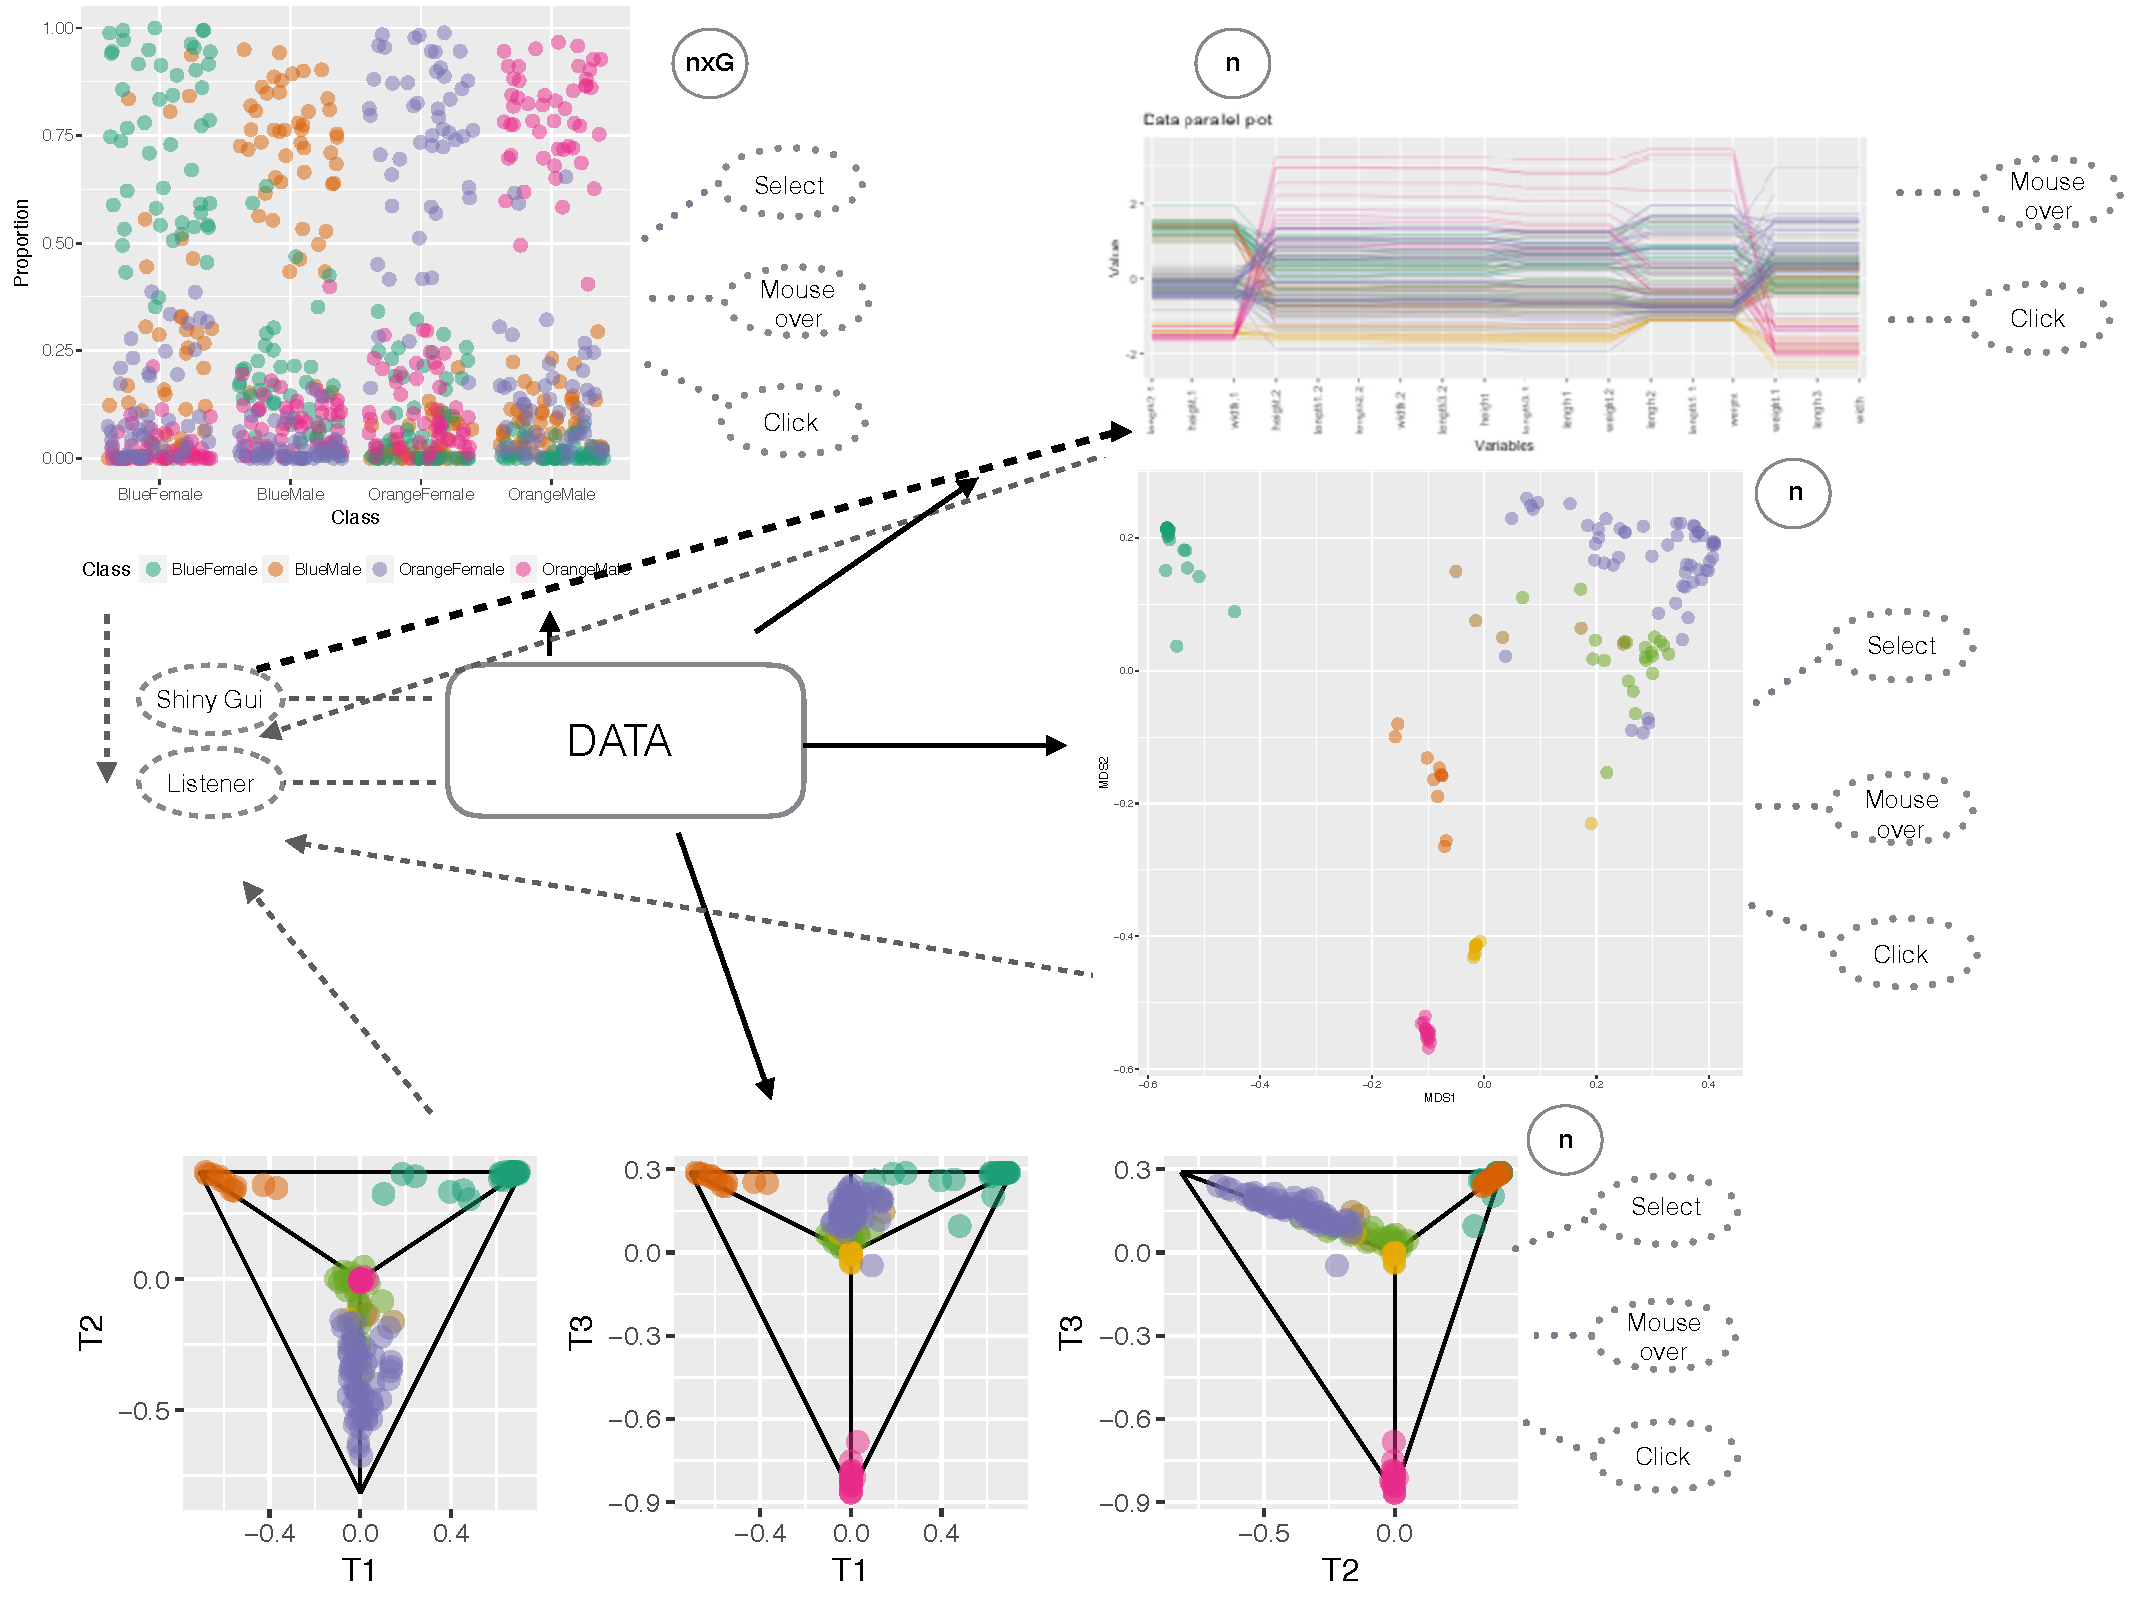
\includegraphics[width=1\linewidth]{figure/fishT1.pdf}
\caption{Schematic diagram illustrating the interactivity in and between plots for individual level exploration panel of the web app. From the data, the four plots are generated. Each plot has a listener attached which collects user actions. When a user selects a point or line in any of the displays, it makes a change in the data which propagates updates to each of the plots.}
\label{tab1diag}
\end{figure}


\subsection{Models}
I have to modify the selection of the tree instead to select the tree based on the importance variable will be better select the tree based on the ooberror. Move the boxplot and select using this one.
This is the only tabset that can not be reproduced using \verb RandomForest  because we don't have the same information than in PPforest. Also doesn't make sense present the 1D projection for each of the node partitions.

This second tab in the app focuses on teasing apart the forest to examine the qualities of each tree. For each tree, information on the variable importance, the projections used at each node, and the oob error is available.  The data feeding into this tab is a list of models along with the original data frame.
The tree id is displayed when we mouse over the jittered side-by-side plot. This information is useful because, based on the accuracy, some trees could be pruned from the forest outside of the app.

Figure \ref{tab2} is a screenshot of the models tab. There are five plots, with varying levels of interaction: (1) a jittered side-by-side dotplot showing variable importance for the top three nodes of all trees in the forest, (2) a static display of one tree, (3) a boxplot of oob error for all trees, (4) a faceted density plot of projected data at each node of the tree, with split point indicated by a vertical line, and (5) a mosaic plot showing the confusion matrix for each node of the tree.  The interaction is driven from the variable importance plot -- when the user selects a point in that display, the corresponding tree density displays and mosaic plots are drawn. The tree plot from the \texttt{PPtreeViz} is used to visualize the selected tree structure. Also highlighted are the variable importance values for each variable for each of the top three nodes and the oob error value for the tree on the boxplot.

% \begin{figure}[hbpt]
% \centering
% \includegraphics[width=1\linewidth]{figure/fish21.png}
% \caption{The individual model tab in the web app. Variable importance is displayed as jittered dot plots for three nodes of all trees. This is linked to a display of the PPTree, a boxplot of the error for all trees in the forest, and display of the data showing splits at each of three nodes and confusion tables as mosaic plots. Clicking a point in the jittered dotplot triggers various updates: each of the importance values for the same tree are highlighted (red), the tree that this corresponds to is drawn, the error for the tree is shown on the boxplot (in red), and the data displays are updated to show the tree. \label{tab2}}
% \end{figure}

The diagram in Figure~\ref{tab2diag} illustrates the data pipeline for interactive graphics.
The data source is a \texttt{PPforest} object. Interaction is driven by the variable importance plot. Selecting a point triggers a change in the data which cascades to re-draws of the other displays. Each plot has some information available on mouse over.

\begin{figure}[hbpt]
\centering
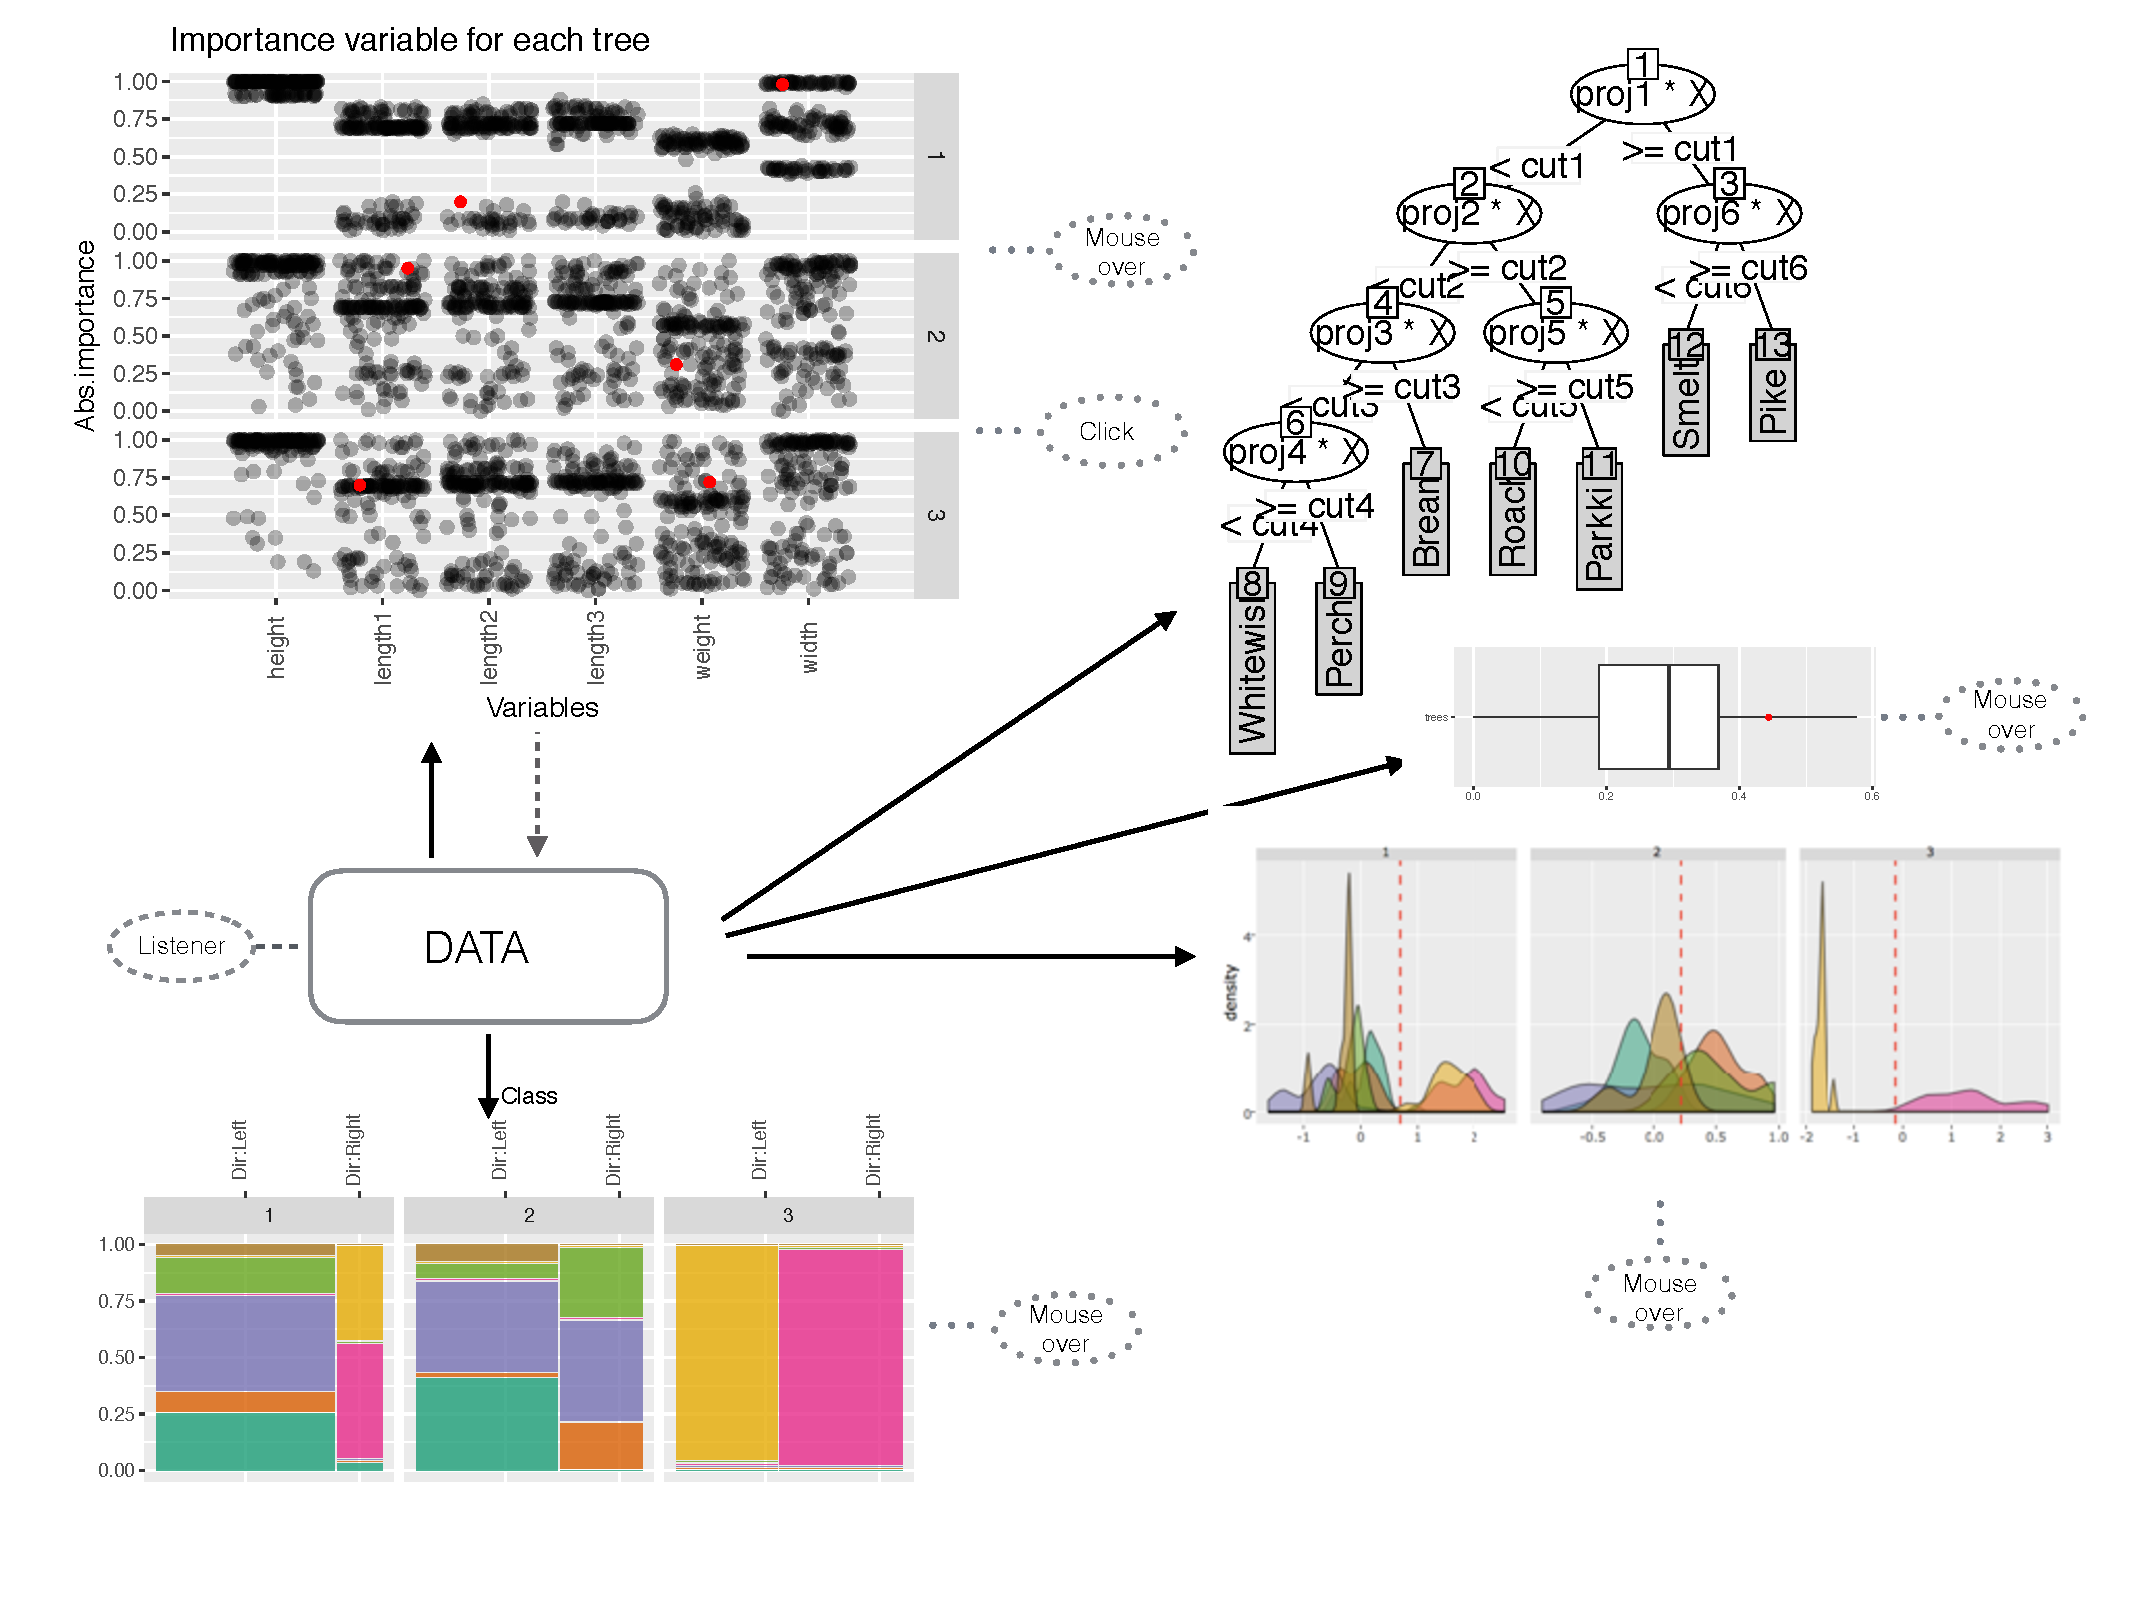
\includegraphics[width=1\linewidth]{figure/fishT2.pdf}
\caption{Schematic diagram illustrating the interactivity in and between plots for model level exploration panel of the web app. Only the dotplot of variable importance is has click selection, which invokes changes of the tree display, boxplot, density plots and mosaic plots. Selecting a point, makes a change in the data, which propagates the importance values for other variables in this tree to be highlighted (red), draws the tree, highlights the error value of the tree, and shows the projections and confusion matrix for the three top nodes.}
\label{tab2diag}
\end{figure}

\subsection{Performance Comparison}

The third tab (see \href{https://natydasilva.shinyapps.io/shinyppforest}{PPforestApp}) examines the PPF fit and compares the result with a RF fit. There are four displays for each type of model: (1) Variable importance for all trees in the forest (same as in the models tab), (2) an receiver operating characteristic curve (ROC) curve comparing sensitivity and specificity for each class, (3) oob error by number of trees to assess complexity, (4) overall variable importance. There is very little interaction on this tab. Users can select to focus on a subset of classes or choose the importance measure to show. Being able to focus on class can help to better understand how well the model performs across classes and the focus can be especially useful for unbalanced data. Examining the oob error by trees enables an assessment of how few trees might be used to provide an equally accurate prediction of future data.

The  ROC is used to summarize the trade-off between sensitivity and specificity. The plot shows the sensitivity and specificity when a parameter of classifier is varied \cite{trevor2011elements}. The specificity and sensitivity was computed with the \texttt{pROC} package.
If more than two classes are available a multi-class ROC analysis is needed. Several solutions have been proposed for multi-class ROC. Some of the proposed reduced the multi-class problem to a set of binary problems. The approach used for a multi-class ROC analysis in this article is called one-against-all \cite{allwein2000reducing}.


% \begin{figure}[hbpt]
% \includegraphics[width=.8\linewidth]{figure/fish31.png}
% \caption{Performance comparison tab of the web app. ROC curves displaying sensitivity against specificity for the classes are shown, along with the oob error by number of trees used to build the forest, and overall variable importance. Displays are shown for the PPF and RF, for comparison purposes. Users can select a class to focus on, using the text entry box. \label{tab3}}
% \end{figure}
%\newpage

\section{Discussion}\label{fur}

Having better tools to open up black box models will provide for better understanding the data, the model strengths and weaknesses, and how the model will performs on future data. This visualization app provides a selection of interactive plots to diagnose PPF models. This shell could be used to make an app for other ensemble classifiers. The philosophy underlying the collection of displays is ``show the model in the data space''  explained in \cite{wickham2015visualizing}. It is not easy to do this, and to completely take this on would require plotting the model in the $p$-dimensional data space. In the simplest approach, as taken here, it means to link the model diagnostics to displays of the data. Then it is possible to probe and query to obtain a better understanding such as finding regions in the data that prove difficult to fit, and detract from the predictive accuracy, or that don't adhere to model assumptions.

The app is implemented with new technology for interactive graphics provided by the \texttt{plotly} package. It is one of the first uses of these new tools.

One challenge to use plotly is that  when layers with different data are created in a ggplot2,  it is difficult to  specify the unique keys required for linking with another plot.

There are many possible extensions to the app, that could help it to be a tool for model refinement: (1) Using the diagnostics to weed out under-performing models in the ensemble; (2) Identifying and boosting models that perform well, particularly if they do well for problematic subsets of the data; (3) Problematic cases could be removed, and ensembles re-fit; (4) Classes as a whole could be aggregated or re-organized as suggested by the model diagnostics, to produce a more effective hierarchical approach to the multiple class problem. Working within the R environment makes all of these desires available using command line outside the app, given the unique ids of models and cases can be exported from the app.

The app has helped to identify ways to improve the  PPtree algorithm and consequently, the PPF model. These especially apply to multiclass problems. Multiple splits for the same class would enable nonlinear classifications. Split criteria tend to place boundaries too close to some groups, due to heteroskedasticity being induced by aggregating classes. Forests are not always better than their constituent trees, and if the trees can be built better, the forest will provide stronger predictions.


\begin{thebibliography}{9}
\bibitem{breiman1996bagging}
Leo Breiman.
\textit{Bagging predictors}
Machine learning.
24(2):123-140,1996.

\bibitem{breiman1984cl}
Leo Breiman, Jerome Friedman, Richard Olshen  and Charles Stone.
\textit{Classification and regression trees}
CRC press,
1984.

\bibitem{BAHM88}
A. Buja, D. Asimov, C. Hurley and J.A. McDonald.
\textit{Elements of a viewing pipeline for data analysis}.
277-308, 1988.

\bibitem{chang11shiny}
Winston Chang,  Joe Cheng, J Allaire, Yihui Xie and Jonathan McPherson.
\textit{shiny: Web application framework for R, R package version 0.11}.
\\\texttt{http://CRAN.R-project.org/package=shiny},
2015.

\bibitem{cutler15raft}
 Adele Cutler and Leo Breiman.
\textit{RAFT: Random forest tool}
\\\texttt{http://www.stat.berkeley.edu/\~{}breiman/RandomForests/cc\_graphics.htm},
2011.

\bibitem{da2021projection}
Natalia da Silva, Dinne Cook and Eun-Kyung Lee.
\textit{A Projection Pursuit Forest Algorithm for Supervised Classification},
Journal of Computational and Graphical Statistics, Taylor \& Francis, 1-21, 2021.


\bibitem{dietterish00}
  Thomas Dietterich.
\textit{Ensemble methods in machine learning},
First International Workshop on Multiple Classifier Systems, Lecture Notes in Computer Science, New York, Springer Verlag, 1-15, 2000.


\bibitem{hurley2011eulerian}
Catherine Hurley and RW Oldford.
\textit{Eulerian tour algorithms for data visualization and the PairViz package}.
Computational Statistics,Springer, 26(4), 613-633, 2011.


\bibitem{Silva2016}
Catarina Silva and Bernardete Ribeiro.
\textit{Visualization of individual ensemble classifier contributions}
Information Processing and Management of Uncertainty in Knowledge-Based Systems: 16th International Conference, IPMU 2016, Eindhoven, The Netherlands, June 20 - 24, 2016, Proceedings, Part II, Springer International Publishing, 633-642, 2016.

\bibitem{lee2013pptree}
Yoon Dong Lee, Dianne  Cook, Ji-won  Park, Eun-Kyung Lee,  and others.
\textit{PPtree: Projection pursuit classification tree}.
Electronic Journal of Statistics, Institute of Mathematical Statistics
7, 1369-1386, 2013.

\bibitem{sutherland2000orca}
Peter Sutherland, Anthony Rossini, Thomas Lumley,  Nicholas  Lewin-Koh, Julie  Dickerson, Zach Cox and Dianne Cook.
 \textit{Orca: A visualization toolkit for high-dimensional data}.
Journal of Computational and Graphical Statistics, Taylor \& Francis, 9(3), 509-529, 2000.



\bibitem{talbot09}
Justin Talbot, Bongshin Lee , Ashish Kapoor and Desney Tan.
\textit{EnsembleMatrix: Interactive visualization to support machine learning with multiple classifiers}.
Proceedings of the SIGCHI Conference on Human Factors in Computing Systems (CHI 09),
Association for Computing Machinery,
New York, NY, USA, 1283-1292, 2009.

\bibitem{quach2012interactive}
Anna Quach.
\textit{Interactive random forests plots}
2012.

\bibitem{RCore}
R Core Team.
\textit{R: A Language and Environment for Statistical Computing}.
R Foundation for Statistical Computing,
\\\texttt{https://www.R-project.org/},
Vienna, Austria, 2016.

\bibitem{CM74}
N. A Campbell and  R. J. Mahon.
\textit{A multivariate study of variation in two species of rock crab of genus Leptograpsus}.
Australian Journal of Zoology, 22, 417-425, 1974.


\bibitem{schloerke}
Barret Schloerke, Hadle Wickham, Dianne Cook,  and Heike Hofmann.
\textit{Escape from Boxland: Generating a library of high-dimensional geometric shapes},
The R Journal,\\\texttt{https://journal.r-project.org/archive/accepted}, 2017.

\bibitem{fishcatch}
  Juha Puranen.
 \textit{Finland fish catch}.
 \\\texttt{https://ww2.amstat.org/publications/jse/jse\_data\_archive.htm}, 2017.



\bibitem{sievertthesis}
Carson Sievert.
\textit{Interfacing R with the web for accessible, portable, and
contents interactive data science}.
ISU repository: \\\texttt{http://lib.dr.iastate.edu/stat\_ag\_etd/}, 2017.


\bibitem{trevor2011elements}
Trevor Hastie, Robert Tibshirani and Jerome Friedman.
\textit{The elements of statistical learning: data mining, inference, and prediction}
Springer, 2011.



\bibitem{plotly}
Carson Sievert, Chris Parmer, Toby Hocking, Scott Chamberlain, Karthik Ram, Marianne Corvellec and Pedro Despouy.
\textit{plotly: Create interactive web-based graphs via plotly's API}.
R package version 1.1.0,
\\\texttt{https://github.com/ropensci/plotly}, 2017.

\bibitem{xie2014reactive}
Yihui Xie, Heike Hofmann, Xiaoyue Cheng and others.
\textit{Reactive programming for interactive graphics}.
Institute of Mathematical Statistics, Statistical Science,
29(2), 201-213, 2014.


\bibitem{sievert2020interactive}
Carson Sievert.
\textit{Interactive web-based data visualization with R, plotly, and shiny}.
CRC Press, 2020. 

\bibitem{urbanek2002exploringold}
Simon Urbanek.
 \textit{Exploring statistical forests}.
Proceedings of the 2002 Joint Statistical Meetings,
2002.

\bibitem{urbanek2002exploring}
Simon Urbanek.
\textit{Visualizing trees and forests}.
Handbook of Data Visualization, Springer Handbooks of Computational Statistics, III.2, 243-264, 2008.

\bibitem{urbanek2011iplots}
Simon Urbanek.
\textit{iPlots eXtreme: next-generation interactive graphics design and implementation of modern interactive graphics}.
Computational Statistics, Springer, 26(3), 381-393, 2011.

\bibitem{allwein2000reducing}
Erin Allwein, Robert SchapireE and Yora Singer.
\textit{Reducing multiclass to binary: A unifying approach for margin classifiers}.
Journal of machine learning research, 1,
Dec, 113-141, 2000.


\bibitem{wickham2015visualizing}
Hadley Wickham, Dianne Cook and Heike Hofmann.
 \textit{Visualizing statistical models: Removing the blindfold}.
Statistical Analysis and Data Mining: The ASA Data Science Journal,
Wiley Online Library, 8(4), 203-225, 2015.


\bibitem{wickham2011tourr}
Hadley Wickham, Dianne Cook, Heike Hofmann, Andres Buja,and others.
\textit{tourr: An R package for exploring multivariate data with projections},
Journal of Statistical Software, American Statistical Association,
40(2), 1-18, 2011.


\bibitem{wickham2009plumbing}
Hadley Wickham,  Michael Lawrence, Dianne Cook, Andreas Buja, Heike Hofmann and Deborah Swayne.
\textit{The plumbing of interactive graphics},
Computational Statistics, Springer,
24(2), 207-215, 2009.


\bibitem{latexcompanion}
Michel Goossens, Frank Mittelbach, and Alexander Samarin.
\textit{The \LaTeX\ Companion}.
Addison-Wesley, Reading, Massachusetts, 1993.

\bibitem{einstein} 
Albert Einstein. 
\textit{Zur Elektrodynamik bewegter K{\"o}rper}. (German) 
[\textit{On the electrodynamics of moving bodies}]. 
Annalen der Physik, 322(10):891-921, 1905.

\bibitem{knuthwebsite} 
Knuth: Computers and Typesetting,
\\\texttt{http://www-cs-faculty.stanford.edu/\~{}uno/abcde.html}
\end{thebibliography}

\end{document}
